\documentclass[14pt, titlepage,fleqn]{extarticle}
\usepackage[T1,T2A]{fontenc}
\usepackage[utf8]{inputenc}

\usepackage{amsmath}
\usepackage[russian]{babel}

\usepackage{titlepage}
\usepackage[final]{pdfpages}
\usepackage{listings}
\usepackage{color}
\usepackage{graphicx}
\usepackage{float} 

\usepackage{caption}


\newcommand{\InsertGraf}[2]{
	\begin{figure}[H]
		\center{\includegraphics[width = 1\textwidth]{#1}}
		\caption{#2}
	\end{figure}
}

\definecolor{dkgreen}{rgb}{0,0.6,0}
\definecolor{gray}{rgb}{0.5,0.5,0.5}
\definecolor{mauve}{rgb}{0.58,0,0.82}


\lstset{frame=single,
	language=Python,
	aboveskip=3mm,
	belowskip=3mm,
	showstringspaces=false,
	columns=flexible,
	basicstyle={\small\ttfamily},
	numbers=none,
	numberstyle=\tiny\color{gray},
	keywordstyle=\color{blue},
	commentstyle=\color{dkgreen},
	stringstyle=\color{mauve},
	breaklines=true,
	breakatwhitespace=true,
	tabsize=3
}

\begin{document}
	\selectlanguage{russian}
	

	\fefutitlepage{Б9119-02.03.01сцт}{Панченко Н.К.}{17}{мая}{22}
	
	
	\newpage
	
 
	\clearpage
	\section*{Постановка задачи}
	Требуется найти минимум функции $f(x) = \dfrac{1}{2}x^TAx + bx$ нескольких переменных при помощи методов Ньютона и градиентного спуска и сравнить результаты и время работы.
	\section*{Решение}
	Данную задачу можно представить системой уравнений:
	\[\begin{cases}
		f_0(x) \rightarrow \min\\
		f(x) \leq 0 
	\end{cases}.\]

	Для поиска оптимального решения воспользуемся теоремой Куна –- Таккера. Из данной теоремы следует, что:
	\begin{enumerate}
		\item $L(x_*, y_*) = \min(L(x,y_* ))$, где $L(x,y_* )=f(x)+y(||x-x_0 ||-r)$,
		\item $y(||x_*-x_0 ||-r)=0 ~~~ (1)$,
		\item $y \geq 0$.
	\end{enumerate}


	Из пункта 2 видно, что возможно два варианта. Если $y=0,$  то мы получаем задачу безусловного минимума, поэтому будем рассматривать только вариант $(||x_*-x_0 ||-r)=0.$


	Так как пространство  $R^n$ является Гильбертовым, $||a||^2=a*a.$ Таким образом,$||x_*-x_0 ||-r $ можно представить как $(x_*-x_0 )*(x_*-x_0 )-r^2.$


	Итак, исходная задача преобразуется в задачу поиска безусловного минимума функции Лагранжа. Получим новое условие минимума:
	\[L' (x,y_* )=f' (x)+2y(x-x_0 )=0~~~ (2)\]
	\newpage
	Решая систему уравнений (1)--(2), получим решение:


	$r$--выбирается из условия, что $||\overline{x} - x_0|| - r > 0$, где $\overline{x}$--точка безусловного минимума.\\


 	Для начала нужно сгенерировать симметричную и положительно определенную матрицу А. Сгенерировав нижнюю треугольную матрицу L, где все элементы на главной диагонали строго больше нуля, и умножив ее на транспонированную матрицу L мы получим необходимую симметрическую и положительно определенную матрицу. В правую часть можно записать любые числа.
	\section*{Реализация алгоритма}
	Для генерации воспользуемся языком программирования Python и библиотекой Numpy для удобной работы с матрицами.
	\begin{lstlisting}
	def pre_generate():
	l = np.zeros((n,n))
	for i in range(n):
		l[i][i] = random.randint(1, 100)
	for i in range(1,n):
		for j in range(i):
			l[i][j] = random.randint(-100, 100)
	b = np.array([random.randint(-100, 100) for i in range(n)])
	a = np.dot(l, np.transpose(l))
	return [a, b]
	\end{lstlisting}


	В обоих методах необходима производная функции, так же в методе Ньютона используется вторая производная.
	\[f(x)=\dfrac{1}{2} x^T Ax+bx\]
	\[f'(x) = \left( \dfrac{1}{2} x^T Ax  \right)' + (bx)' = \dfrac{1}{2}\left(A+ A^T \right)x+b=Ax+b\]
	\[f''(x)= (Ax)' + b' = A\]


	Для метода Ньютона необходимо нахождение обратной матрицы. Будем искать обратную матрицу с помощью матрицы из алгебраических дополнений.
	\section*{Реализация алгоритма}
	\begin{lstlisting}
def det(a):
	if(type(a[0]) != list or len(a) != len(a[0])):
		return None
	if(len(a) == 2):
		return a[0][0] * a[1][1] - a[0][1]*a[1][0]
	elif(len(a) == 3):
		sum = 0
		for i in range(3):
			p = 1
			m = 1
			for j in range(3):
				p *= a[(i + j)%3][j]
				m *= a[(i + j)%3][2-j]
			sum += p
			sum -= m
		return sum
	else:
		sum = 0
		for i in range(len(a)):
			sum += (-1)**i * a[0][i]*det(minor(a,i,0))
		return sum

def minor(a,x,y):
	to_ret = []
	for r in a:
		temp = r[:]
		temp.pop(x)
		to_ret += [temp]
	to_ret.pop(y)
	return to_ret

def inv(a):
	c = [r[:] for r in a]
	for i in range(len(a)):
		for j in range(len(a[0])):
			c[i][j] = (-1)**(i + j)*det(minor(a,j,i))
	return mul(transpose(c),1/det(a))

	\end{lstlisting}


	\section*{Метод Ньютона}
	Поиск значений x для нахождения минимума функции осуществляется по следующей формуле:
	\[x^{k+1} = x^k - \dfrac{f'(x^k)}{f''(x^k)}\]
	В нашем случае начальные значения x не влияют на ход работы и для вычисления значений x потребуется лишь одна итерация, потому как:
	\[x^1 = x^0 - \dfrac{f'(x^0)}{f''(x^0)}= x^0 - A^{-1}(Ax^0 + b) = x^0 - A^{-1}Ax^0 - A^{-1}b = - A^{-1}b\]
	Тогда подставив в производную найденные значения получим, что мы нашли стационарную точку, являющуюся минимумом функции:
	\[f'(x^1) = Ax^{1} + b = A(-A^{-1}b) + b = -b +b =0\]
	Вычисления происходили бы не за один шаг, если бы у нас была другая функция, соответственно другие производные.



	\section*{Реализация алгоритма}
	Для реализации воспользуемся языком программирования Python и библиотекой Numpy для удобной работы с матрицами.
	%[title=dwdw, captionpos=b]
	\begin{lstlisting}
		def newtons_method(x,a,b):
	return x - dot(inv(a), dfunc(x,a,b))
	\end{lstlisting}
	В обоих методах необходима производная функции, так же в методе Ньютона используется вторая производная.
	

	
	\section*{Метод градиентного спуска}
	Поиск значений x для нахождения минимума функции осуществляется по следующей формуле:
	\[x^{k+1} = x^k - \lambda f'(x^k)\]
	Будем брать $\lambda = 10^{-6}$, а вычисления проводить до тех пор, пока разница между значениями функций $f(x^k)$ и $f(x^{k+1})$ будет больше, чем $10^{-10}$.


	\section*{Реализация алгоритма}
	Для реализации воспользуемся языком программирования Python и библиотекой Numpy для удобной работы с матрицами.
	\begin{lstlisting}
	def grad_method(x,a,b,step = 0.0001):
	xn = [r[:] for r in x]
	while(step > 0.000000001):
		start = func(xn,a,b)
		d = dfunc(xn,a,b)
		right  = mul(d ,-step)
		xn = plus(xn, right)
		end = func(xn,a,b)
		if(start < end):
			step /= 10
	return xn

	\end{lstlisting}

	В обоих методах необходима производная функции, так же в методе Ньютона используется вторая производная.
	



	\newpage
	\section*{Тесты}
	\begin{figure}[H]
		\center{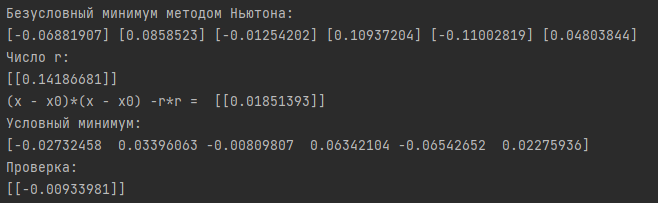
\includegraphics[width = 1\textwidth]{lb2.png}}
	\end{figure}


	\newpage
	\section*{Заключение}
	Таким образом в данной лабораторной работе я реализовал и изучил метод Ньютона и градиентного спуска для поиска минимального значения функции нескольких переменных и провел тесты работы методов, из которых видно, что:
	\begin{enumerate}
		\item Размер матрицы сильно влияет на время работы метода градиентного спуска
		\item Начальные данные влияют на скорость работы и количество итераций метода градиентного спуска.
	\end{enumerate}
\end{document}